\chapter{Experiments and Results}
\label{experiments-and-results}

Each experiment has a hypothesis, a setup and a result.

\section{Hardware}
For the purpose of this thesis we had access to two machines. The smaller machine is a personal machine and a large machine rented at the provider Exoscale \cite{noauthor_exoscale_nodate}. They will be referred to as \textit{Balthazar} and \textit{Melchior} respectively. Their specifications are described in table \ref{hardware}.

\begin{table*}
    \begin{center}
        \begin{tabular}{ c|c|c }
            Component & Balthazar             & Melchior                \\
            \hline
            \hline
            CPU       & 6 Core AMD Ryzen 3600 & 24 Core Intel Broadwell \\
            RAM       & 32GB                  & 120GB                   \\
            GPU       & NVIDIA GTX 1660 Super & 3 $\cdot$ NVIDIA P100   \\
            VRAM      & 6GB                   & 3 $\cdot$ 16GB          \\
            Storage   & 500GB SSD             & 400GB SSD               \\
        \end{tabular}
    \end{center}
    \caption{Hardware specifications of the utilized machines}
    \label{hardware}
\end{table*}

\section{Parameters}
\label{parameters}
The behavior of the system is controlled by a multitude of parameters. The most relevant parameters are listed in table \ref{parameters}. If one of the parameters differs from the default values in an experiment, it will be mentioned. For each experiment, all parameters are pesisted by the system.

\begin{table}
    \begin{center}
        \begin{tabularx}{\textwidth}{ c|c|X }
            Name                       & Default   & Explanation                                                                                   \\
            \hline
            \hline
            temp\_treshhold            & 60        & The number of moves for which the next move is sampled (cf. equation \ref{eq:move_selection}) \\
            update\_treshold           & 0.6       & The percentage of matches, that has to be won for a new network to be accepted                \\
            num\_MCTS\_sims            & 120       & The number of times the search tree is expanded during MCTS                                   \\
            num\_self\_play\_workers   & 9         & The number of workers used for parallel self-play                                             \\
            num\_arena\_workers        & 8         & The number of workers used for parallel Arena matches                                         \\
            load\_model                & false     & Indicates whether to load an existing model                                                   \\
            maxlen\_experience\_buffer & 1,000,000 & The maximum number of tuples ($s, \pi, z$) in the buffer                                      \\
            nnet\_size                 & mini      & The neural net used as introduced in \ref{neural_network_architecture}                        \\
            lr                         & 0.001     & The learning rate during training of the neural network                                       \\
            epochs                     & 10        & The number of of epochs during training of the neural network                                 \\
            batch\_size                & 64        & The size of the batches during training of the neural network                                 \\
        \end{tabularx}
    \end{center}
    \caption{The parameters of the training pipeline}
    \label{parameter_table}
\end{table}

\section{Validation}
\paragraph{Hypothesis} The modified framework still converges to optimal play for TicTacToe.
\paragraph{Setup} Run pipeline with modified implemenation of TicTacToe from \cite{thakoor_suragnairalpha-zero-general_nodate} on Balthazar.
\begin{table}[!h]
    \begin{center}
        \begin{tabular}{ c|c }
            Name                       & Value   \\
            \hline
            \hline
            temp\_treshhold            & 15      \\
            num\_MCTS\_sims            & 30      \\
            num\_self\_play\_workers   & 2       \\
            num\_arena\_workers        & 2       \\
            maxlen\_experience\_buffer & 960,000 \\
        \end{tabular}
    \end{center}
    \caption{The parameters for the validation runs}
\end{table}
\paragraph{Result} Convergence to optimal play given for TicTacToe (cf. figure \ref{tictactoe_performance}).

\begin{figure}
    \centering
    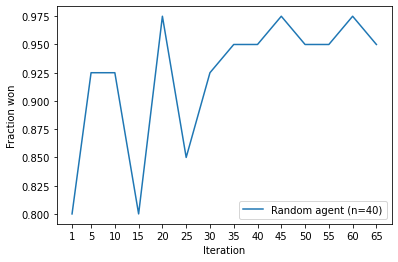
\includegraphics[height=6cm, keepaspectratio]{validation_tictactoe.png}
    \caption{Wins against random baseline in TicTacToe. Win ratio is $\frac{\text{gamesWon}}{\text{allGames}}$ }
    \label{tictactoe_performance}
\end{figure}

\section{Application}
\subsection{Naive Run}
\paragraph{Hypothesis} The naive implementation without any Abalone specific modifications converges to optimal play.
\paragraph{Setup} Run pipeline on Balthazar.
\paragraph{Result} No improvement in playing performance, cf. figure \ref{performance_local_naive}
\begin{figure}[!h]
    \centering
    \subfloat[The win-ratio of the naive implementation]{
        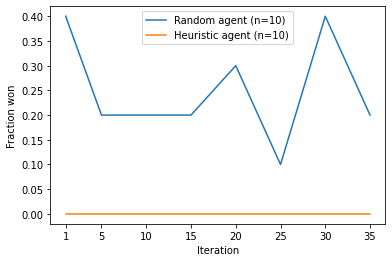
\includegraphics[height=5cm, keepaspectratio]{performance_local_win_ratio.png}
    }
    \hfill
    \subfloat[The cumulative reward recieved by the naive implementation]{
        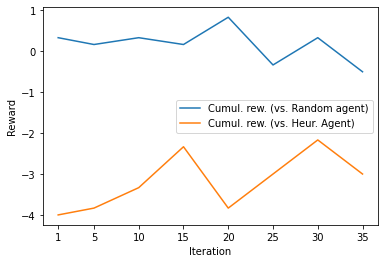
\includegraphics[height=5cm, keepaspectratio]{performance_local_reward.png}
    }
    \caption{}
    \label{performance_local_naive}
\end{figure}

\subsection{Scaled naive Run}
\paragraph{Hypothesis} The naive implementation without any Abalone specific modifications converges to optimal play on a larger machine with a bigger buffer and more workers.
\paragraph{Setup} Run pipeline on Melchior.
\paragraph{Result} No improvement in playing performance, divergence, cf. figure \ref{performance_remote_naive}
\begin{figure}[!h]
    \centering
    \subfloat[The win-ratio of the naive implementation]{
        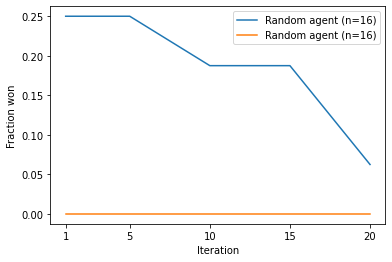
\includegraphics[height=5cm, keepaspectratio]{performance_remote_naive_win_ratio.png}
    }
    \hfill
    \subfloat[The cumulative reward recieved by the naive implementation]{
        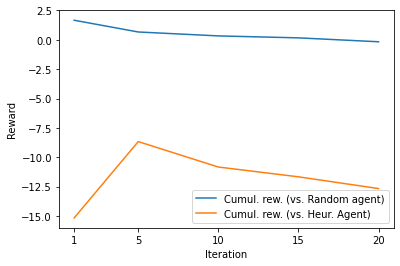
\includegraphics[height=5cm, keepaspectratio]{performance_remote_naive_reward.png}
    }
    \caption{}
    \label{performance_remote_naive}
\end{figure}

\subsection{Reward Distribution}
\paragraph{Hypothesis} The distribution of game results $z$ is uneven.
\paragraph{Setup} Plot histogram of $z$ in buffer of previous run.
\paragraph{Result} Most of the games end up as drawn or with minor advantage for one player, cf. figure \ref{distribution_of_rewards}).

\begin{figure}
    \centering
    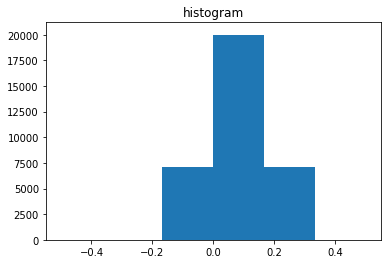
\includegraphics[height=6cm, keepaspectratio]{distribution_of_z.png}
    \caption{Distribution of $z$ in experience buffer}
    \label{distribution_of_rewards}
\end{figure}

\subsection{Scaled warmed-up Run}
\paragraph{Hypothesis} Pretraining the network on experience generated by Verloop's minimax against a random player nudges the network towards more aggressive play. The resulting experience buffer has stronger signals $z$, which improves performance.
\paragraph{Setup} Run pipeline on Melchior with pretrained network.
\paragraph{Result}
\begin{figure}[!h]
    \centering
    \subfloat[The win-ratio of the naive implementation]{
        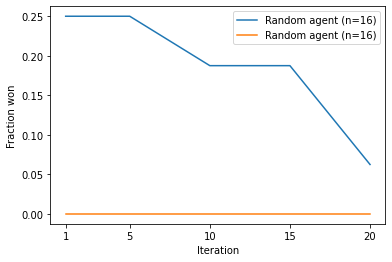
\includegraphics[height=5cm, keepaspectratio]{performance_remote_naive_win_ratio.png}
    }
    \hfill
    \subfloat[The cumulative reward recieved by the naive implementation]{
        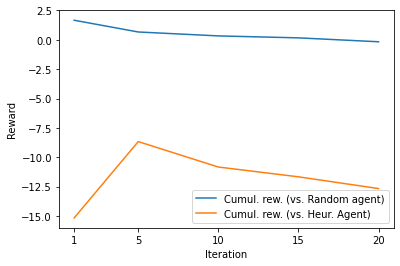
\includegraphics[height=5cm, keepaspectratio]{performance_remote_naive_reward.png}
    }
    \caption{}
    \label{performance_remote_warmed_up}
\end{figure}

\subsection{Scaled Run with adjusted Reward $z$}
\paragraph{Hypothesis} Pretraining the network on experience generated by Verloop's minimax against a random player nudges the network towards more aggressive play. The resulting experience buffer has stronger signals $z$, which improves performance.
\paragraph{Setup} Run pipeline on Melchior with pretrained network.
\paragraph{Result}
\begin{figure}[!h]
    \centering
    \subfloat[The win-ratio of the naive implementation]{
        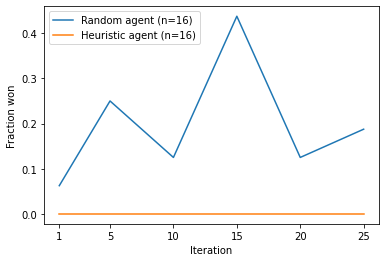
\includegraphics[height=5cm, keepaspectratio]{performance_remote_diff_z_win_ratio.png}
    }
    \hfill
    \subfloat[The cumulative reward recieved by the naive implementation]{
        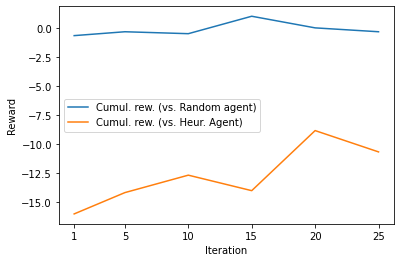
\includegraphics[height=5cm, keepaspectratio]{performance_remote_diff_z_cumul_reward.png}
    }
    \caption{}
    \label{performance_remote_diff_z}
\end{figure}